\documentclass[11pt,border=6pt]{standalone}
\usepackage{fontspec}
\usepackage{tikz}
\begin{document}
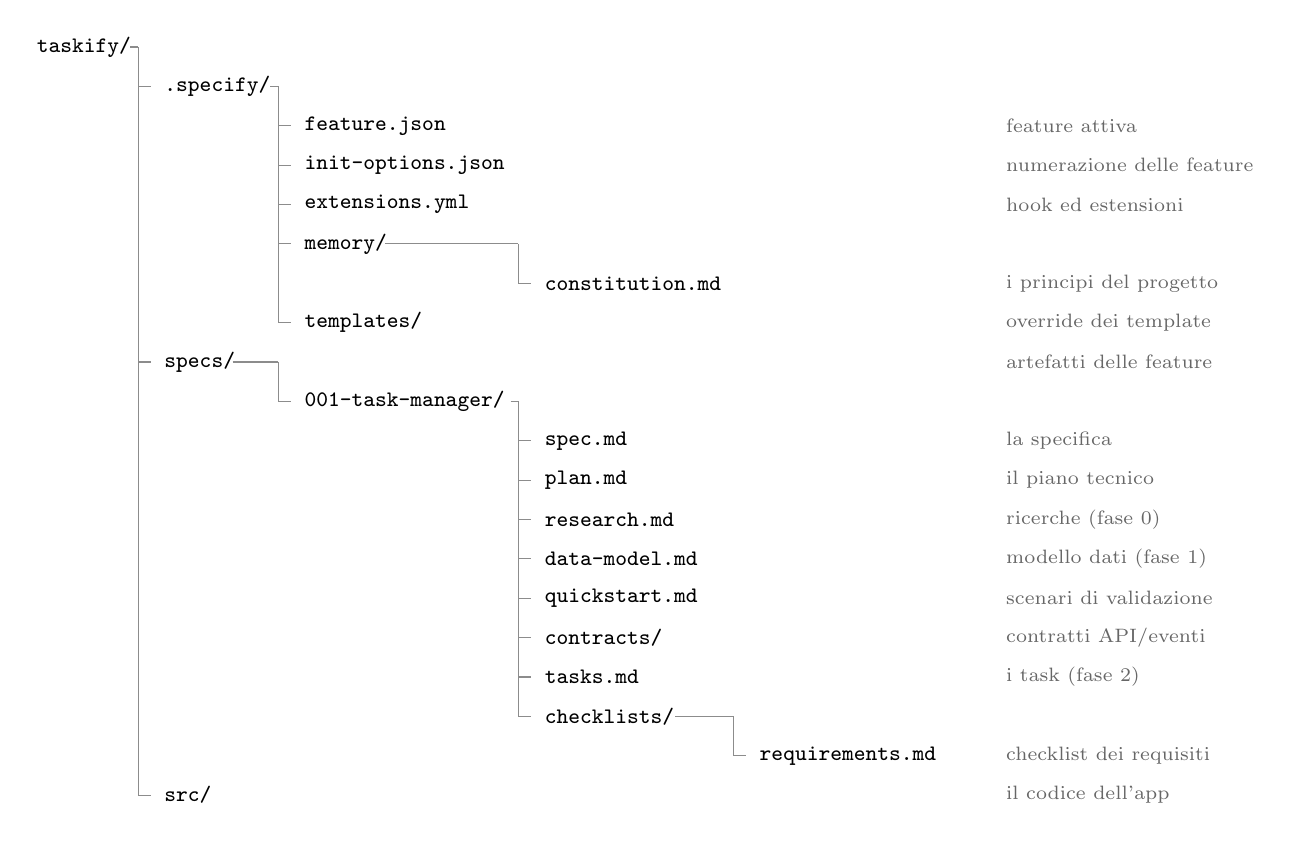
\begin{tikzpicture}

% nodi: nome in monospazio, annotazione in grigio
\node[anchor=west, font=\ttfamily\footnotesize] (n0) at (0.00,0.00) {taskify/};
\node[anchor=west, font=\ttfamily\footnotesize] (n1) at (1.62,-0.50) {.specify/};
\node[anchor=west, font=\ttfamily\footnotesize] (n2) at (3.40,-1.00) {feature.json};
\node[anchor=west, font=\scriptsize, text=black!60] at (12.31,-1.00) {feature attiva};
\node[anchor=west, font=\ttfamily\footnotesize] (n3) at (3.40,-1.50) {init-options.json};
\node[anchor=west, font=\scriptsize, text=black!60] at (12.31,-1.50) {numerazione delle feature};
\node[anchor=west, font=\ttfamily\footnotesize] (n4) at (3.40,-2.00) {extensions.yml};
\node[anchor=west, font=\scriptsize, text=black!60] at (12.31,-2.00) {hook ed estensioni};
\node[anchor=west, font=\ttfamily\footnotesize] (n5) at (3.40,-2.50) {memory/};
\node[anchor=west, font=\ttfamily\footnotesize] (n6) at (6.45,-3.00) {constitution.md};
\node[anchor=west, font=\scriptsize, text=black!60] at (12.31,-3.00) {i principi del progetto};
\node[anchor=west, font=\ttfamily\footnotesize] (n7) at (3.40,-3.50) {templates/};
\node[anchor=west, font=\scriptsize, text=black!60] at (12.31,-3.50) {override dei template};
\node[anchor=west, font=\ttfamily\footnotesize] (n8) at (1.62,-4.00) {specs/};
\node[anchor=west, font=\scriptsize, text=black!60] at (12.31,-4.00) {artefatti delle feature};
\node[anchor=west, font=\ttfamily\footnotesize] (n9) at (3.40,-4.50) {001-task-manager/};
\node[anchor=west, font=\ttfamily\footnotesize] (n10) at (6.45,-5.00) {spec.md};
\node[anchor=west, font=\scriptsize, text=black!60] at (12.31,-5.00) {la specifica};
\node[anchor=west, font=\ttfamily\footnotesize] (n11) at (6.45,-5.50) {plan.md};
\node[anchor=west, font=\scriptsize, text=black!60] at (12.31,-5.50) {il piano tecnico};
\node[anchor=west, font=\ttfamily\footnotesize] (n12) at (6.45,-6.00) {research.md};
\node[anchor=west, font=\scriptsize, text=black!60] at (12.31,-6.00) {ricerche (fase 0)};
\node[anchor=west, font=\ttfamily\footnotesize] (n13) at (6.45,-6.50) {data-model.md};
\node[anchor=west, font=\scriptsize, text=black!60] at (12.31,-6.50) {modello dati (fase 1)};
\node[anchor=west, font=\ttfamily\footnotesize] (n14) at (6.45,-7.00) {quickstart.md};
\node[anchor=west, font=\scriptsize, text=black!60] at (12.31,-7.00) {scenari di validazione};
\node[anchor=west, font=\ttfamily\footnotesize] (n15) at (6.45,-7.50) {contracts/};
\node[anchor=west, font=\scriptsize, text=black!60] at (12.31,-7.50) {contratti API/eventi};
\node[anchor=west, font=\ttfamily\footnotesize] (n16) at (6.45,-8.00) {tasks.md};
\node[anchor=west, font=\scriptsize, text=black!60] at (12.31,-8.00) {i task (fase 2)};
\node[anchor=west, font=\ttfamily\footnotesize] (n17) at (6.45,-8.50) {checklists/};
\node[anchor=west, font=\ttfamily\footnotesize] (n18) at (9.18,-9.00) {requirements.md};
\node[anchor=west, font=\scriptsize, text=black!60] at (12.31,-9.00) {checklist dei requisiti};
\node[anchor=west, font=\ttfamily\footnotesize] (n19) at (1.62,-9.50) {src/};
\node[anchor=west, font=\scriptsize, text=black!60] at (12.31,-9.50) {il codice dell'app};

% connettori ad albero
\draw[black!45] (1.31,0.00) -- (1.41,0.00);
\draw[black!45] (1.41,0.00) -- (1.41,-9.50);
\draw[black!45] (1.41,-0.50) -- (1.57,-0.50);
\draw[black!45] (1.41,-4.00) -- (1.57,-4.00);
\draw[black!45] (1.41,-9.50) -- (1.57,-9.50);
\draw[black!45] (3.09,-0.50) -- (3.19,-0.50);
\draw[black!45] (3.19,-0.50) -- (3.19,-3.50);
\draw[black!45] (3.19,-1.00) -- (3.35,-1.00);
\draw[black!45] (3.19,-1.50) -- (3.35,-1.50);
\draw[black!45] (3.19,-2.00) -- (3.35,-2.00);
\draw[black!45] (3.19,-2.50) -- (3.35,-2.50);
\draw[black!45] (3.19,-3.50) -- (3.35,-3.50);
\draw[black!45] (4.55,-2.50) -- (6.24,-2.50);
\draw[black!45] (6.24,-2.50) -- (6.24,-3.00);
\draw[black!45] (6.24,-3.00) -- (6.40,-3.00);
\draw[black!45] (2.61,-4.00) -- (3.19,-4.00);
\draw[black!45] (3.19,-4.00) -- (3.19,-4.50);
\draw[black!45] (3.19,-4.50) -- (3.35,-4.50);
\draw[black!45] (6.14,-4.50) -- (6.24,-4.50);
\draw[black!45] (6.24,-4.50) -- (6.24,-8.50);
\draw[black!45] (6.24,-5.00) -- (6.40,-5.00);
\draw[black!45] (6.24,-5.50) -- (6.40,-5.50);
\draw[black!45] (6.24,-6.00) -- (6.40,-6.00);
\draw[black!45] (6.24,-6.50) -- (6.40,-6.50);
\draw[black!45] (6.24,-7.00) -- (6.40,-7.00);
\draw[black!45] (6.24,-7.50) -- (6.40,-7.50);
\draw[black!45] (6.24,-8.00) -- (6.40,-8.00);
\draw[black!45] (6.24,-8.50) -- (6.40,-8.50);
\draw[black!45] (8.23,-8.50) -- (8.97,-8.50);
\draw[black!45] (8.97,-8.50) -- (8.97,-9.00);
\draw[black!45] (8.97,-9.00) -- (9.13,-9.00);
\end{tikzpicture}
\end{document}
